\documentclass[graphics]{beamer}

\usepackage{graphicx}
\usepackage{verbatim}
\usepackage{wrapfig}
\useoutertheme{shadow}
%\usecolortheme{orchid}
\usecolortheme{seahorse}


% math commands
\newcommand{\be}{\begin{eqnarray}}
\newcommand{\ee}{\end{eqnarray}}
\newcommand{\beq}{\begin{equation}}
\newcommand{\eeq}{\end{equation}}
\def\simless{\mathbin{\lower 3pt\hbox
      {$\rlap{\raise 5pt\hbox{$\char'074$}}\mathchar"7218$}}}
\def\simgreat{\mathbin{\lower 3pt\hbox
      {$\rlap{\raise 5pt\hbox{$\char'076$}}\mathchar"7218$}}} %> or of order

% variables

\def\toonscale{0.45}
\def\mboxy#1{\mbox{\small #1}}


\begin{comment}
\AtBeginSection[]{
  \frame{
    \frametitle{Outline}
    \tableofcontents[currentsection]
  }
}
\end{comment}

\title{Precision Measurements of Space and Time
}
\subtitle{}
\author[U. Pen]{Ue-Li Pen
\\[8mm] 
}
\date{Sept 13, 2016}


\begin{document}


\begin{comment}
  \subsection{Outline}

  \frame{
    \frametitle{Outline}
    \tableofcontents
  }
\end{comment}
\frame{\maketitle}

  \frame{
\vspace{-0.5in}
    \frametitle{Topics}
    \begin{itemize}
        \item scintillometry, FRB's
        \item pulsar tests of gravity
        \item LSS: 21cm (theory, CHIME, GBT, Parkes), tides, neutrinos
        \item HPC: SciNet (GPC, LP), SOSCIP (BGQ, FPGA, LM), TH2++
        \item Fluids
    \end{itemize}
  }

  \frame{
    \frametitle{Fluids}
    \begin{itemize}
      \item w/N. Turok, 1510.02985, PRL in press
      \item cosmic adiabatic perturbations of amplitude $\epsilon$
        turn into shock waves at scales $\epsilon$ of the horizon scale
      \item generate subhorizon gravitational waves through Cherenkov
        radiation, potentially probe PBH with PTA
        \item work in progress w/Feldbrugge, Inman, Schnetter, Turok
    \end{itemize}
\vspace{-0.6in}\hspace{.1in}
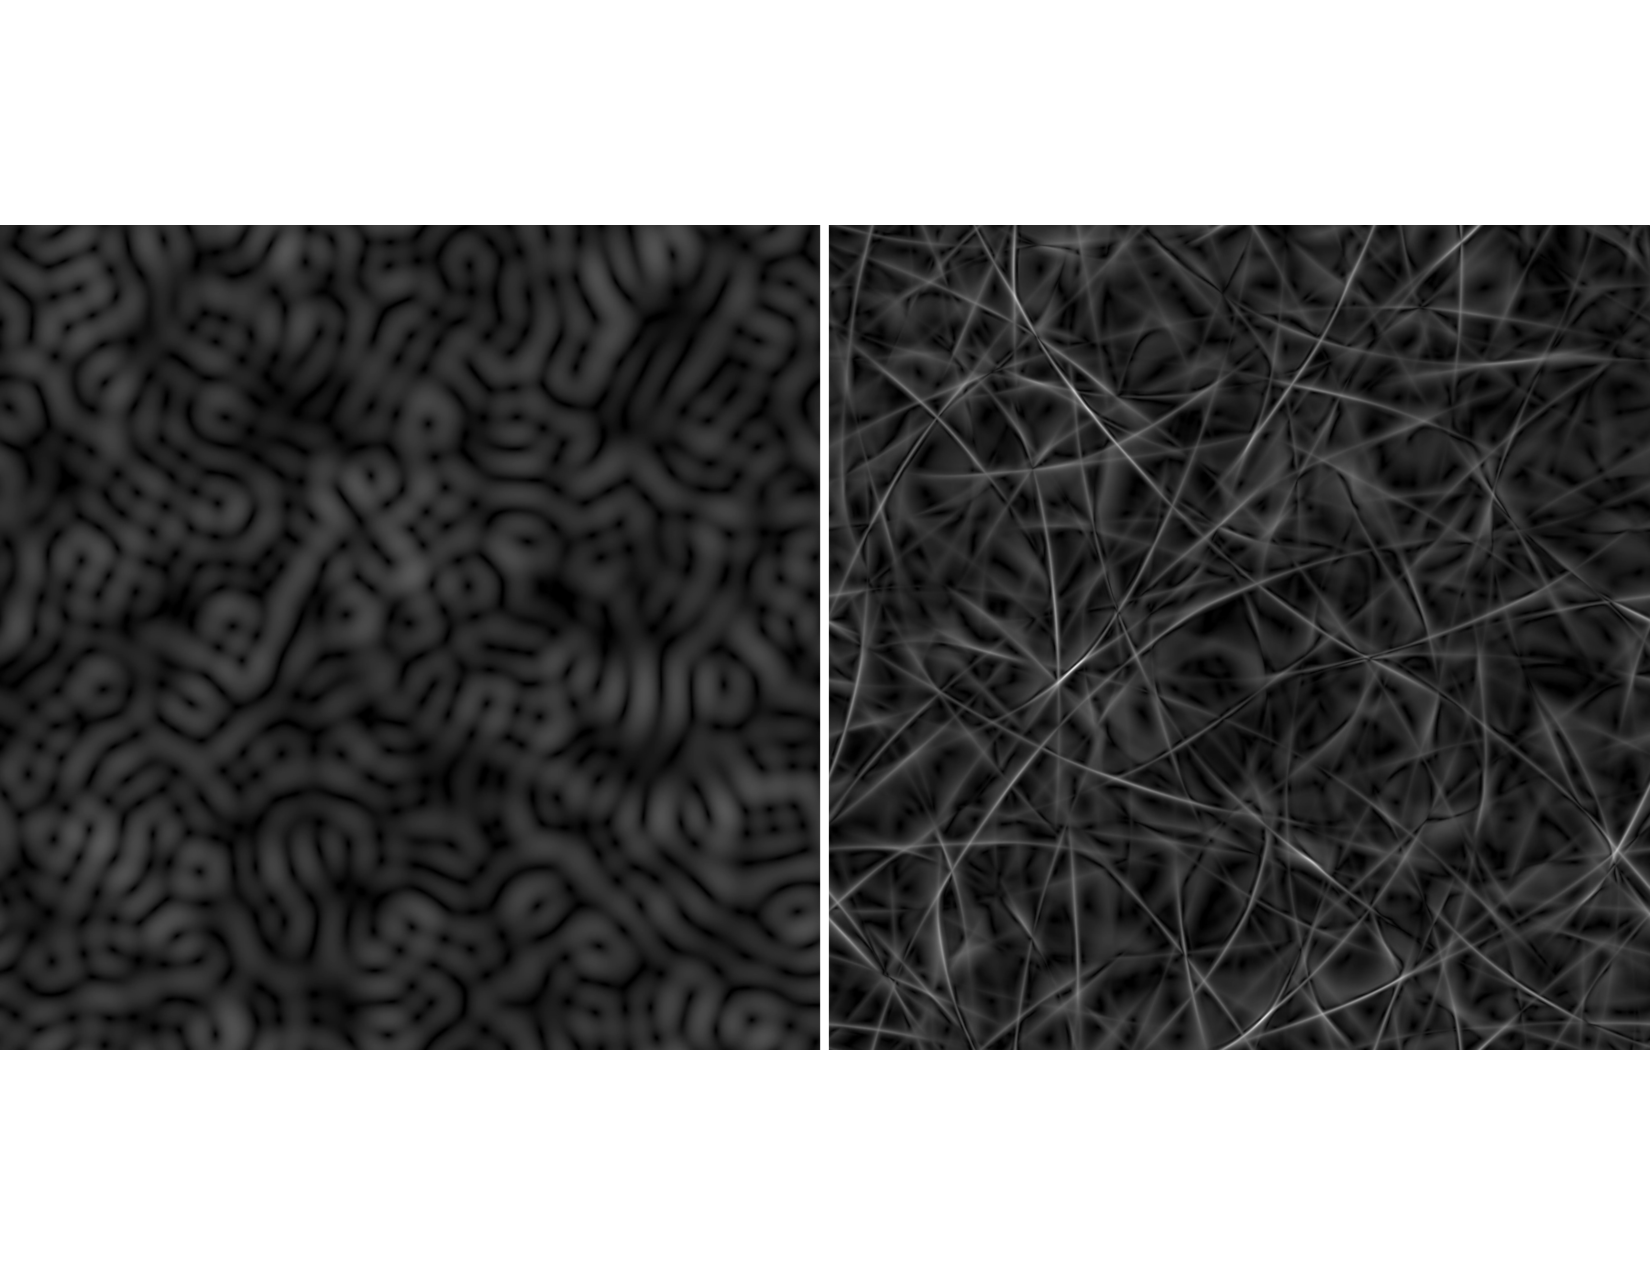
\includegraphics[width=4in]{Figures/shockspanel1.pdf}
%\vspace{-0.5in}
}

\end{document}
